\documentclass[12pt]{article}
\usepackage{times}
\usepackage[english]{babel}
\usepackage[utf8x]{inputenc}
\usepackage[colorinlistoftodos]{todonotes}
\usepackage[margin=1in]{geometry}
\usepackage{graphicx}
\usepackage{epstopdf}
\usepackage{cite}
\usepackage{listings}
\usepackage{dtklogos}
\usepackage{wrapfig}
\usepackage{subfigure}
\usepackage{amsmath}
\usepackage{amsthm}
\usepackage{amssymb}
\usepackage{amscd}
\usepackage{caption}
\usepackage{etoolbox}
\usepackage{fancyhdr}
\usepackage{stackengine}
\usepackage[export]{adjustbox}
\patchcmd{\thebibliography}{\section*{\refname}}{}{}{}
\usepackage[document]{ragged2e}    %This causes text to left align
\usepackage[colorlinks=true, linkcolor=black,citecolor=black,urlcolor=blue]{hyperref}
\bibliographystyle{IEEEtran}
\DeclareGraphicsRule{.tif}{png}{.png}{`convert #1 `dirname #1`/`basename #1 .tif`.png}

\title{MCHE 474: Lab 6}

\begin{document}
\lefthyphenmin3
\righthyphenmin4
% \pretolerance=2000
% \tolerance=500 
% \emergencystretch=10pt
%\raggedright     %Stops LaTeX from automatically hyphenating the right margin to fit better
%Combine this with \usepackage[document]{ragged2e} to get a text align left similar to natural MS Word


%-------------------------------------------------------------
%Start of Paper
%-------------------------------------------------------------

%%%%%%%%%%%%%%%%%%%%%%%%%%%%%%%%%%%%%%%%%%%%%%%%%%%%%%
%%%%%%%%%%%%%%%%%%%%%%% TITLE PAGE %%%%%%%%%%%%%%%%%%%%%%%%
%%%%%%%%%%%%%%%%%%%%%%%%%%%%%%%%%%%%%%%%%%%%%%%%%%%%%%

\begin{titlepage}

\newcommand{\HRule}{\rule{\linewidth}{0.5mm}} % Defines a new command for the horizontal lines, change thickness here

\center % Center everything on the page
 
%----------------------------------------------------------------------------------------
%	Heading Section
%----------------------------------------------------------------------------------------

\textsc{\LARGE University of Louisiana at Lafayette}\\[1.5cm] % Name of your university/college
\textsc{\Large Control Systems}\\[0.5cm] % Major heading such as course name
\textsc{\large MCHE 474}\\[0.5cm] % Minor heading such as course title

%----------------------------------------------------------------------------------------
%	Title Section
%----------------------------------------------------------------------------------------

\HRule \\[0.4cm]
{ \huge \bfseries Lab 6}\\[0.4cm] % Title of your document
\HRule \\[1.5cm]
 
%----------------------------------------------------------------------------------------
%	Author Section
%----------------------------------------------------------------------------------------

\begin{minipage}{0.4\textwidth}
\begin{flushleft} \large
\emph{Author:}\\
\textsc{Matthew J. Begneaud} \\% Your name
\end{flushleft}
\end{minipage}
~
\begin{minipage}{0.4\textwidth}
\begin{flushright} \large
\emph{Professor:} \\
\textsc{Dr. Mostafa A. Elsayed} % Supervisor's Name
\end{flushright}
\end{minipage}\\[1.5cm]

% If you don't want a supervisor, uncomment the two lines below and remove the section above
%\Large \emph{Author:}\\
%John \textsc{Smith}\\[3cm] % Your name

%----------------------------------------------------------------------------------------
%	Date Section
%----------------------------------------------------------------------------------------

{\textsc{\large \today}}\\[2cm] % Date, change the \today to a set date if you want to be precise

%----------------------------------------------------------------------------------------
%	Logo Section
%----------------------------------------------------------------------------------------


\includegraphics[width=5in]{UL_logo.jpg}\\[1cm] % Include a department/university logo - this will require the graphicx package
 
%----------------------------------------------------------------------------------------

\vfill % Fill the rest of the page with whitespace

\end{titlepage}

%%%%%%%%%%%%%%%%%%%%%%%%%%%%%%%%%%%%%%%%%%%%%%%%%%%%%%
%%%%%%%%%%%%%%%%%%%%%%% TABLE OF CONTENTS %%%%%%%%%%%%%%%%%%%
%%%%%%%%%%%%%%%%%%%%%%%%%%%%%%%%%%%%%%%%%%%%%%%%%%%%%%

\tableofcontents

\listoffigures

\section*{\fontsize{12}{12}\selectfont \large List of Symbols}
\addcontentsline{toc}{section}{List of Symbols} % Add for each section
$G$ = System plant \\
$G_{c}$ = System controller \\
$H$ = System feedback \\
$T$ = Transfer Function \\
$K$ = Controller gain \\
$K_{cr}$ = Critical gain \\


\newpage

%%%%%%%%%%%%%%%%%%%%%%%%%%%%%%%%%%%%%%%%%%%%%%%%%%%%%%
%%%%%%%%%%%%%%%%%%%%%%% REPORT %%%%%%%%%%%%%%%%%%%%%%%%%%
%%%%%%%%%%%%%%%%%%%%%%%%%%%%%%%%%%%%%%%%%%%%%%%%%%%%%%


\section*{\fontsize{12}{12}\selectfont \large Introduction}
\addcontentsline{toc}{section}{Introduction} % Add for each section
This lab was conducted using MATLAB to analyze a control system. The system?s plant is given in Equation 1, the controller in Equation 2, and the negative feedback in Equation 3. The system's critical gain $K$ at the limit of stability is found using the RH criterion. The root-locus is then plotted by hand, as well as the Bode plot. The gain margin and phase margin are found using the Bode plot and the gain margin is compared to the value calculated using the RH criterion. The system root-locus and Bode plots were then plotted in MATLAB and the system step response when $K = 0.5K_{cr}$ was plotted and performance criteria was calculated.
\bigskip

\begin{equation}
G = \frac{s + 10}{s(s^2 + 3s + 25)}
\end{equation}

\begin{equation}
G_{c} = K
\end{equation}

\begin{equation}
H = -1
\end{equation}



\section*{\fontsize{12}{12}\selectfont \large Theory}
\addcontentsline{toc}{section}{Theory} % Add for each section
The root-locus plot of a system can reveal much about the behavior of the system. The root-locus is a plot showing the location of zeros and poles of the system. Zeros of a system are the values of s that cause the numerator of the transfer function to equal zero. Poles are the values of s that cause the denominator of the transfer function to equal zero. The zeros and poles of a system are often times complex numbers. For this reason, the root-locus plot of a system is plotted on the real-imaginary plane. The root-locus plot shows how the poles and zeros change as an applied gain K goes from 0 to $\infty$.
\bigskip

A Bode plot is a plot of the system's amplitude and phase at different input frequencies. The amplitude is typically expressed in Decibels (dB) and the frequency is typically expressed in logarithmic increments. The Bode plot contains two plots: the amplitude plot, and the phase plot. 



\section*{\fontsize{12}{12}\selectfont \large Procedure \& Analysis}
\addcontentsline{toc}{section}{Procedure \& Analysis} % Add for each section
The transfer function of the system was first defined, shown in Equation 4. As shown in Figure 1, the RH criterion was then used to find $K_{cr}$ at the limit of stability and the root locus was plotted by hand. The Bode plot was also plotted by hand, as seen in Figure 2 and Figure 3. 
\bigskip

\begin{equation}
T = \frac{K}{s(s^2 + 3s + 25) + K}
\end{equation}

\newpage

% Figure 1: hand drawn root locus and RH calculations 
\begin{figure}[h!] %  figure placement: here, top, bottom, or page
   \centering
   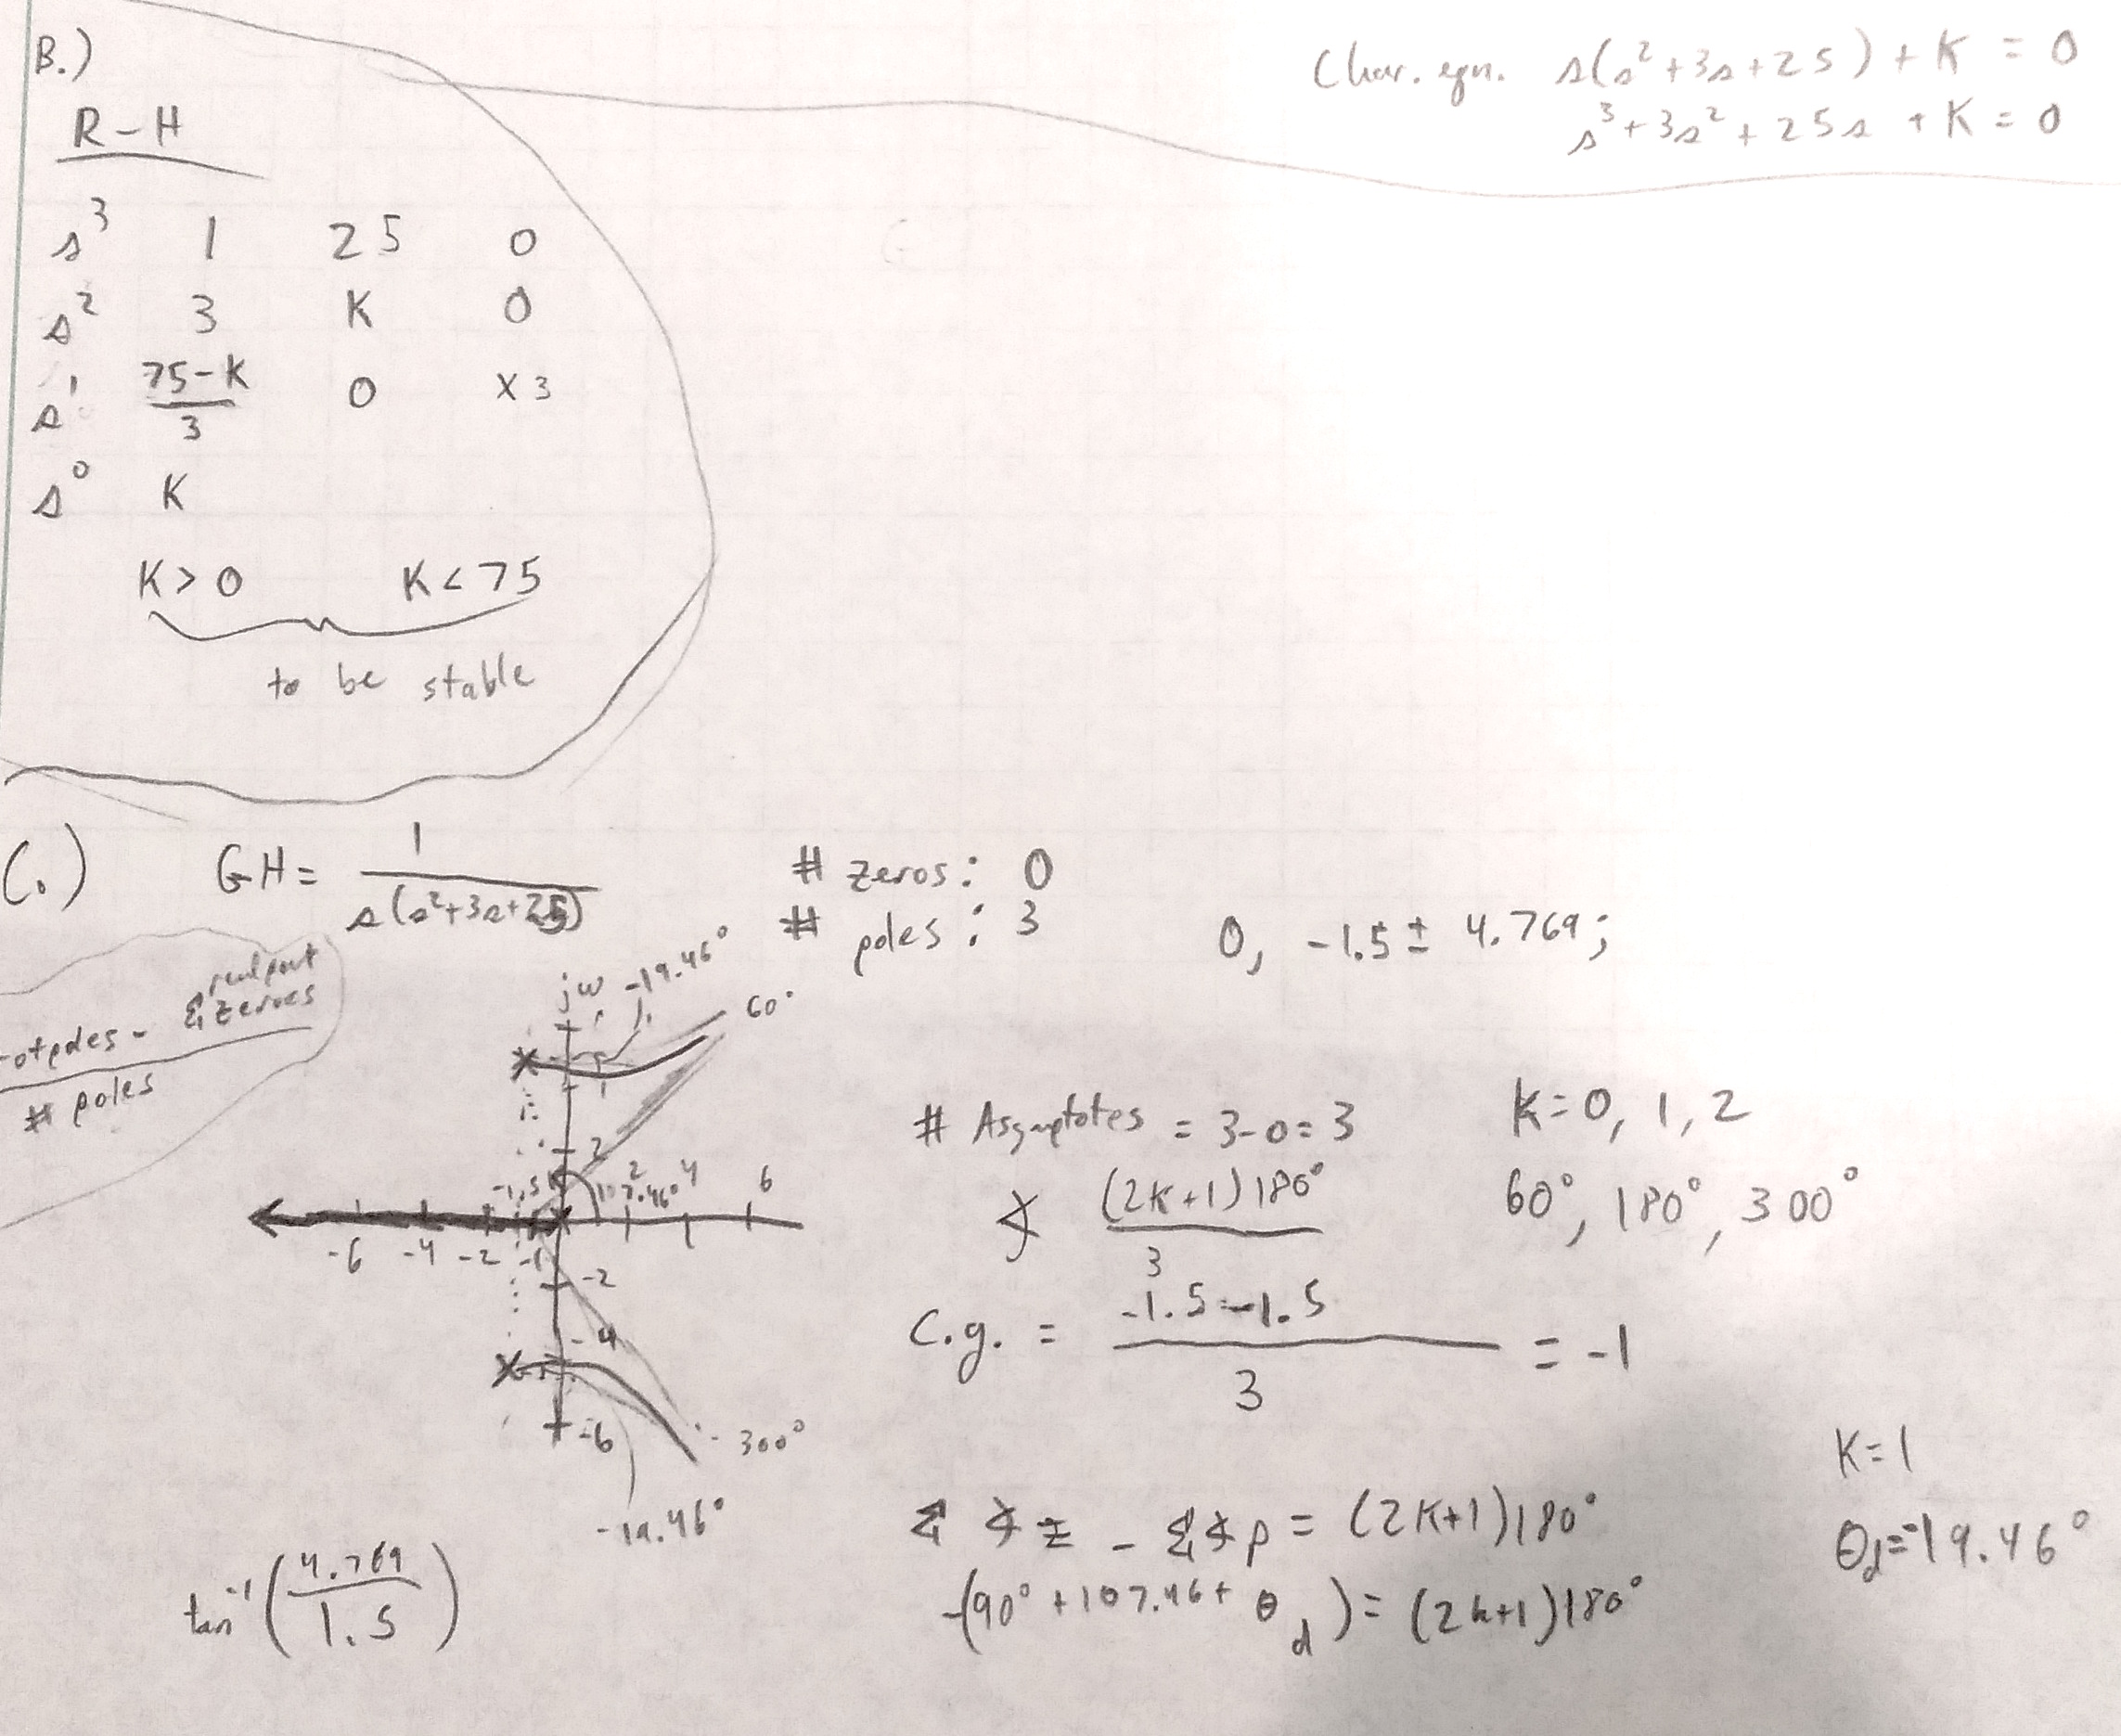
\includegraphics[width=4.5in]{hand_drawn_root_locus.jpg} 
   \caption{Hand Performed RH Criterion and Root Locus Plot}
   \label{fig:example}
\end{figure}

% Figure 2: hand drawn Bode Plot mag
\begin{figure}[h!] %  figure placement: here, top, bottom, or page
   \centering
   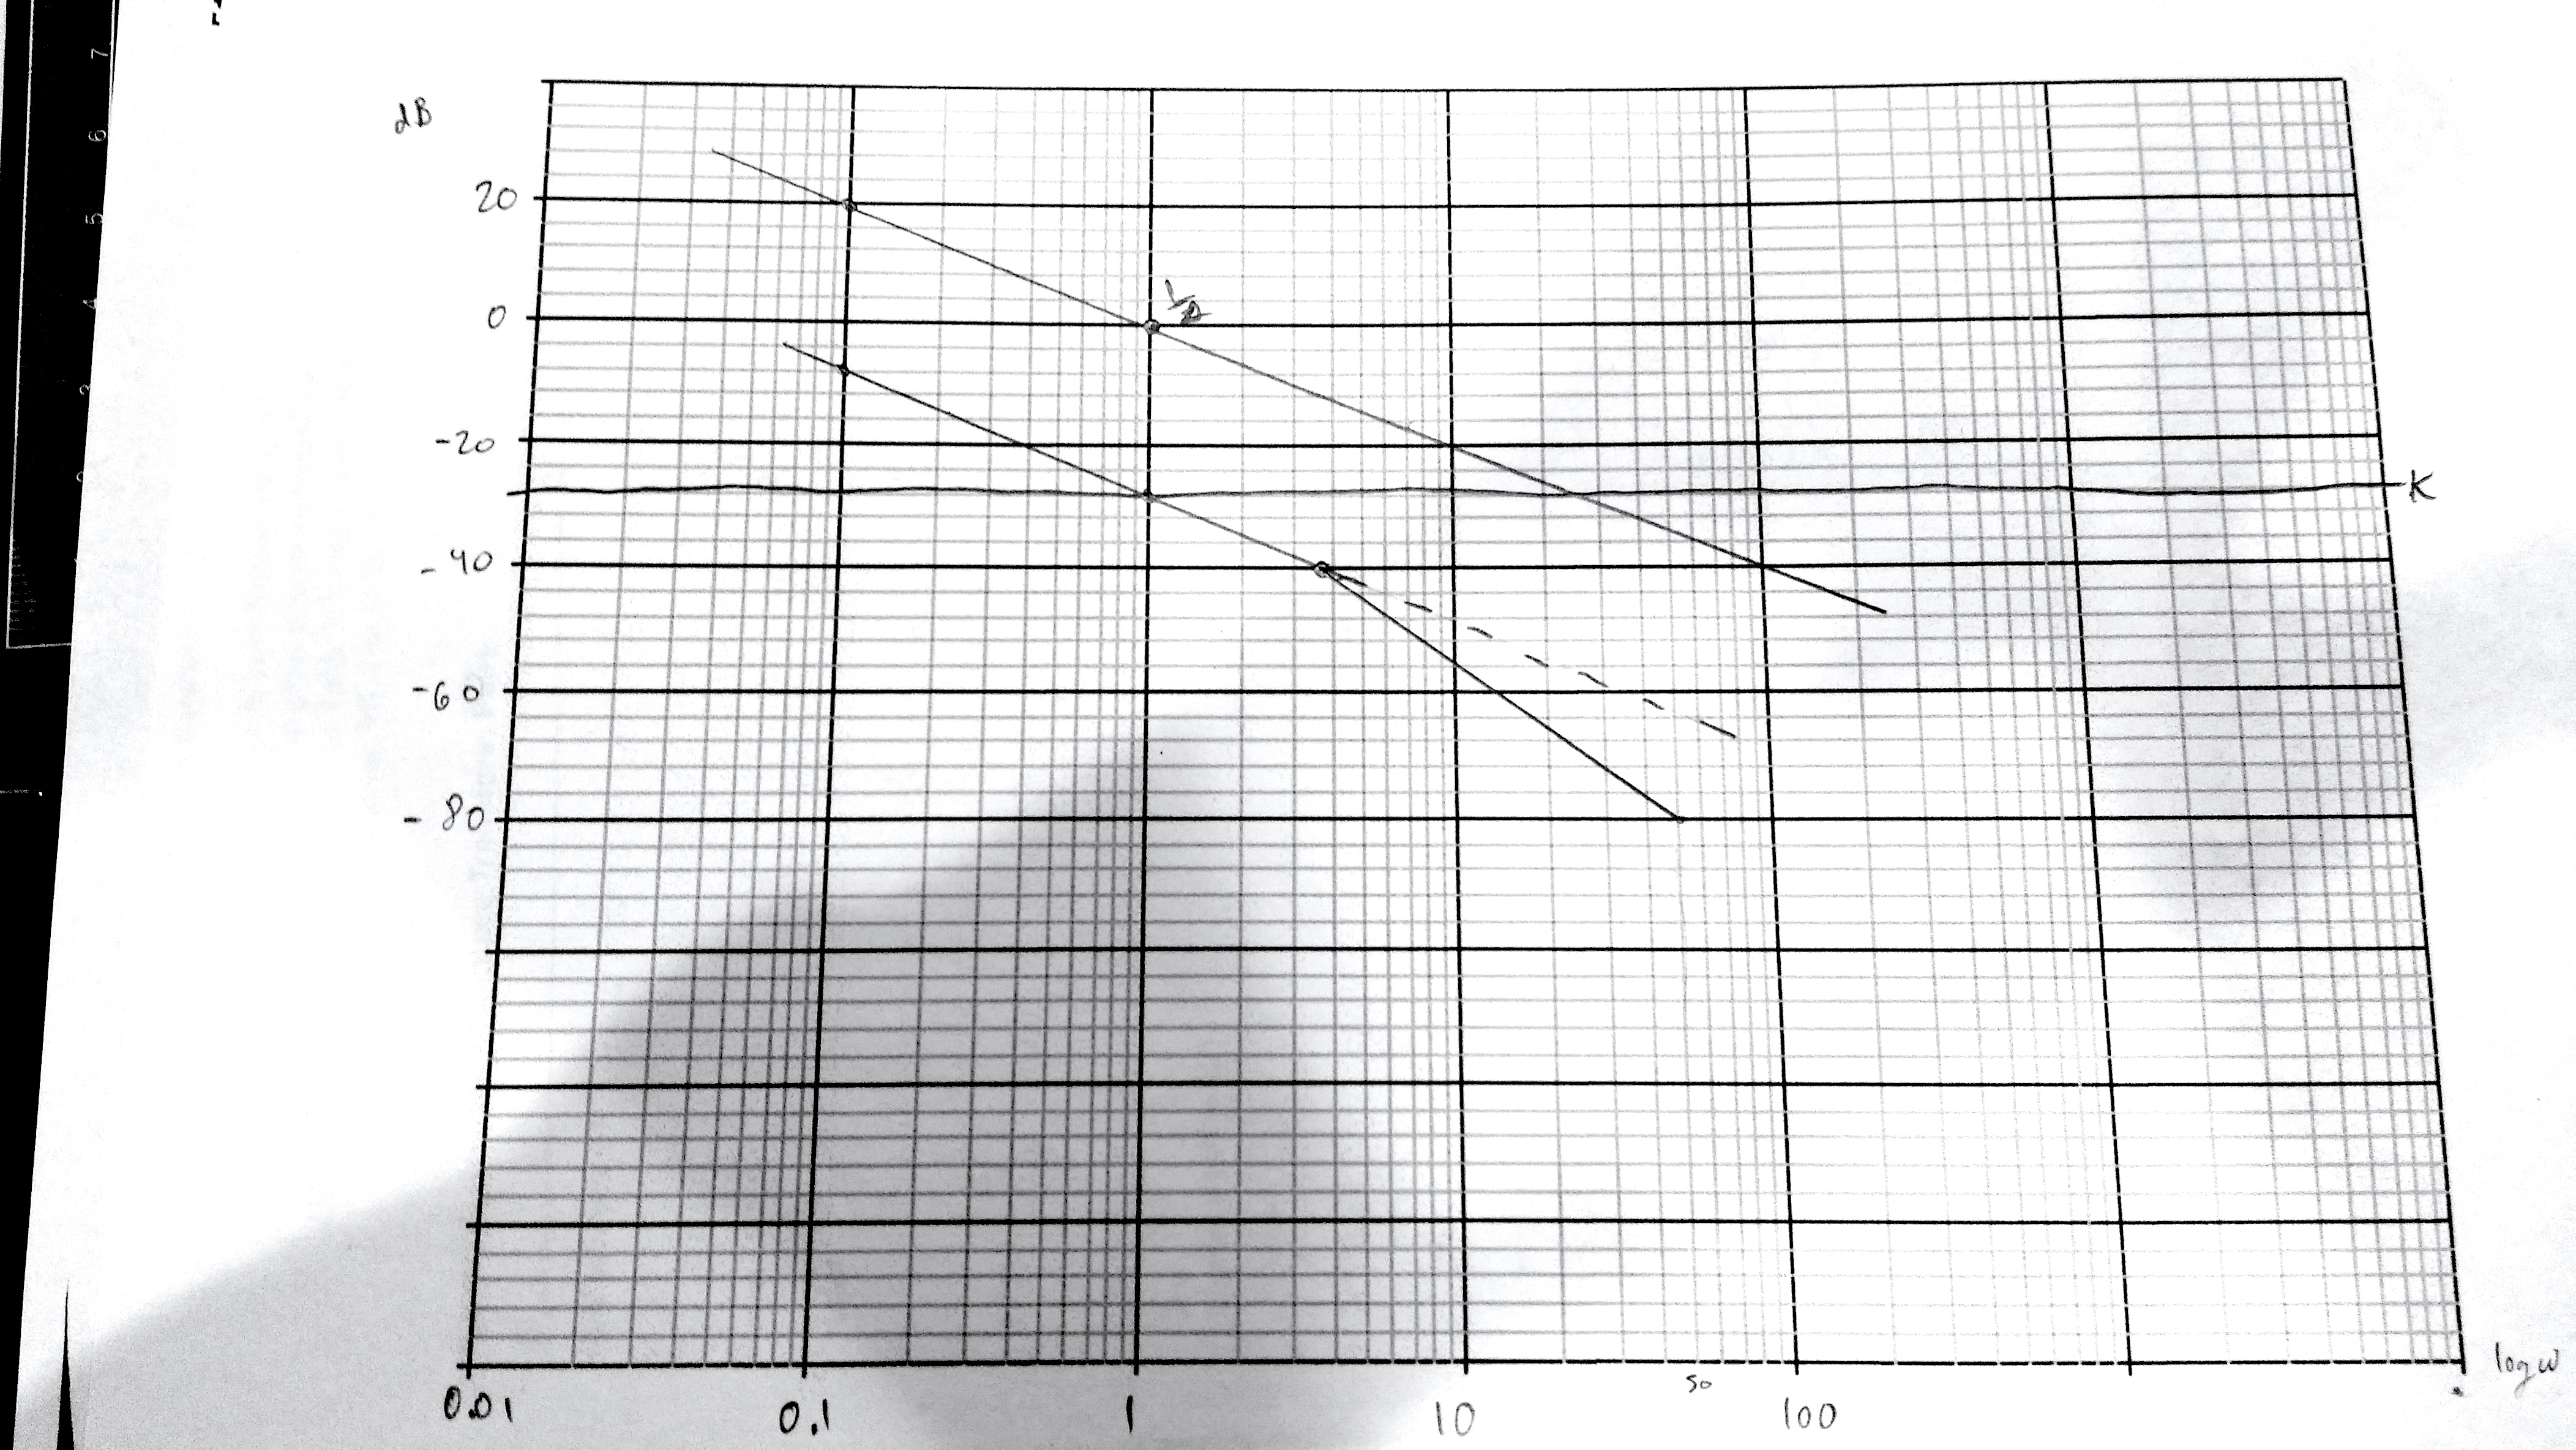
\includegraphics[width=6in]{hand_drawn_bode_plot_magnitude.jpg} 
   \caption{Hand Performed Bode Plot Magnitude}
   \label{fig:example}
\end{figure}

\newpage

% Figure 3: hand drawn Bode Plot freq
\begin{figure}[h!] %  figure placement: here, top, bottom, or page
   \centering
   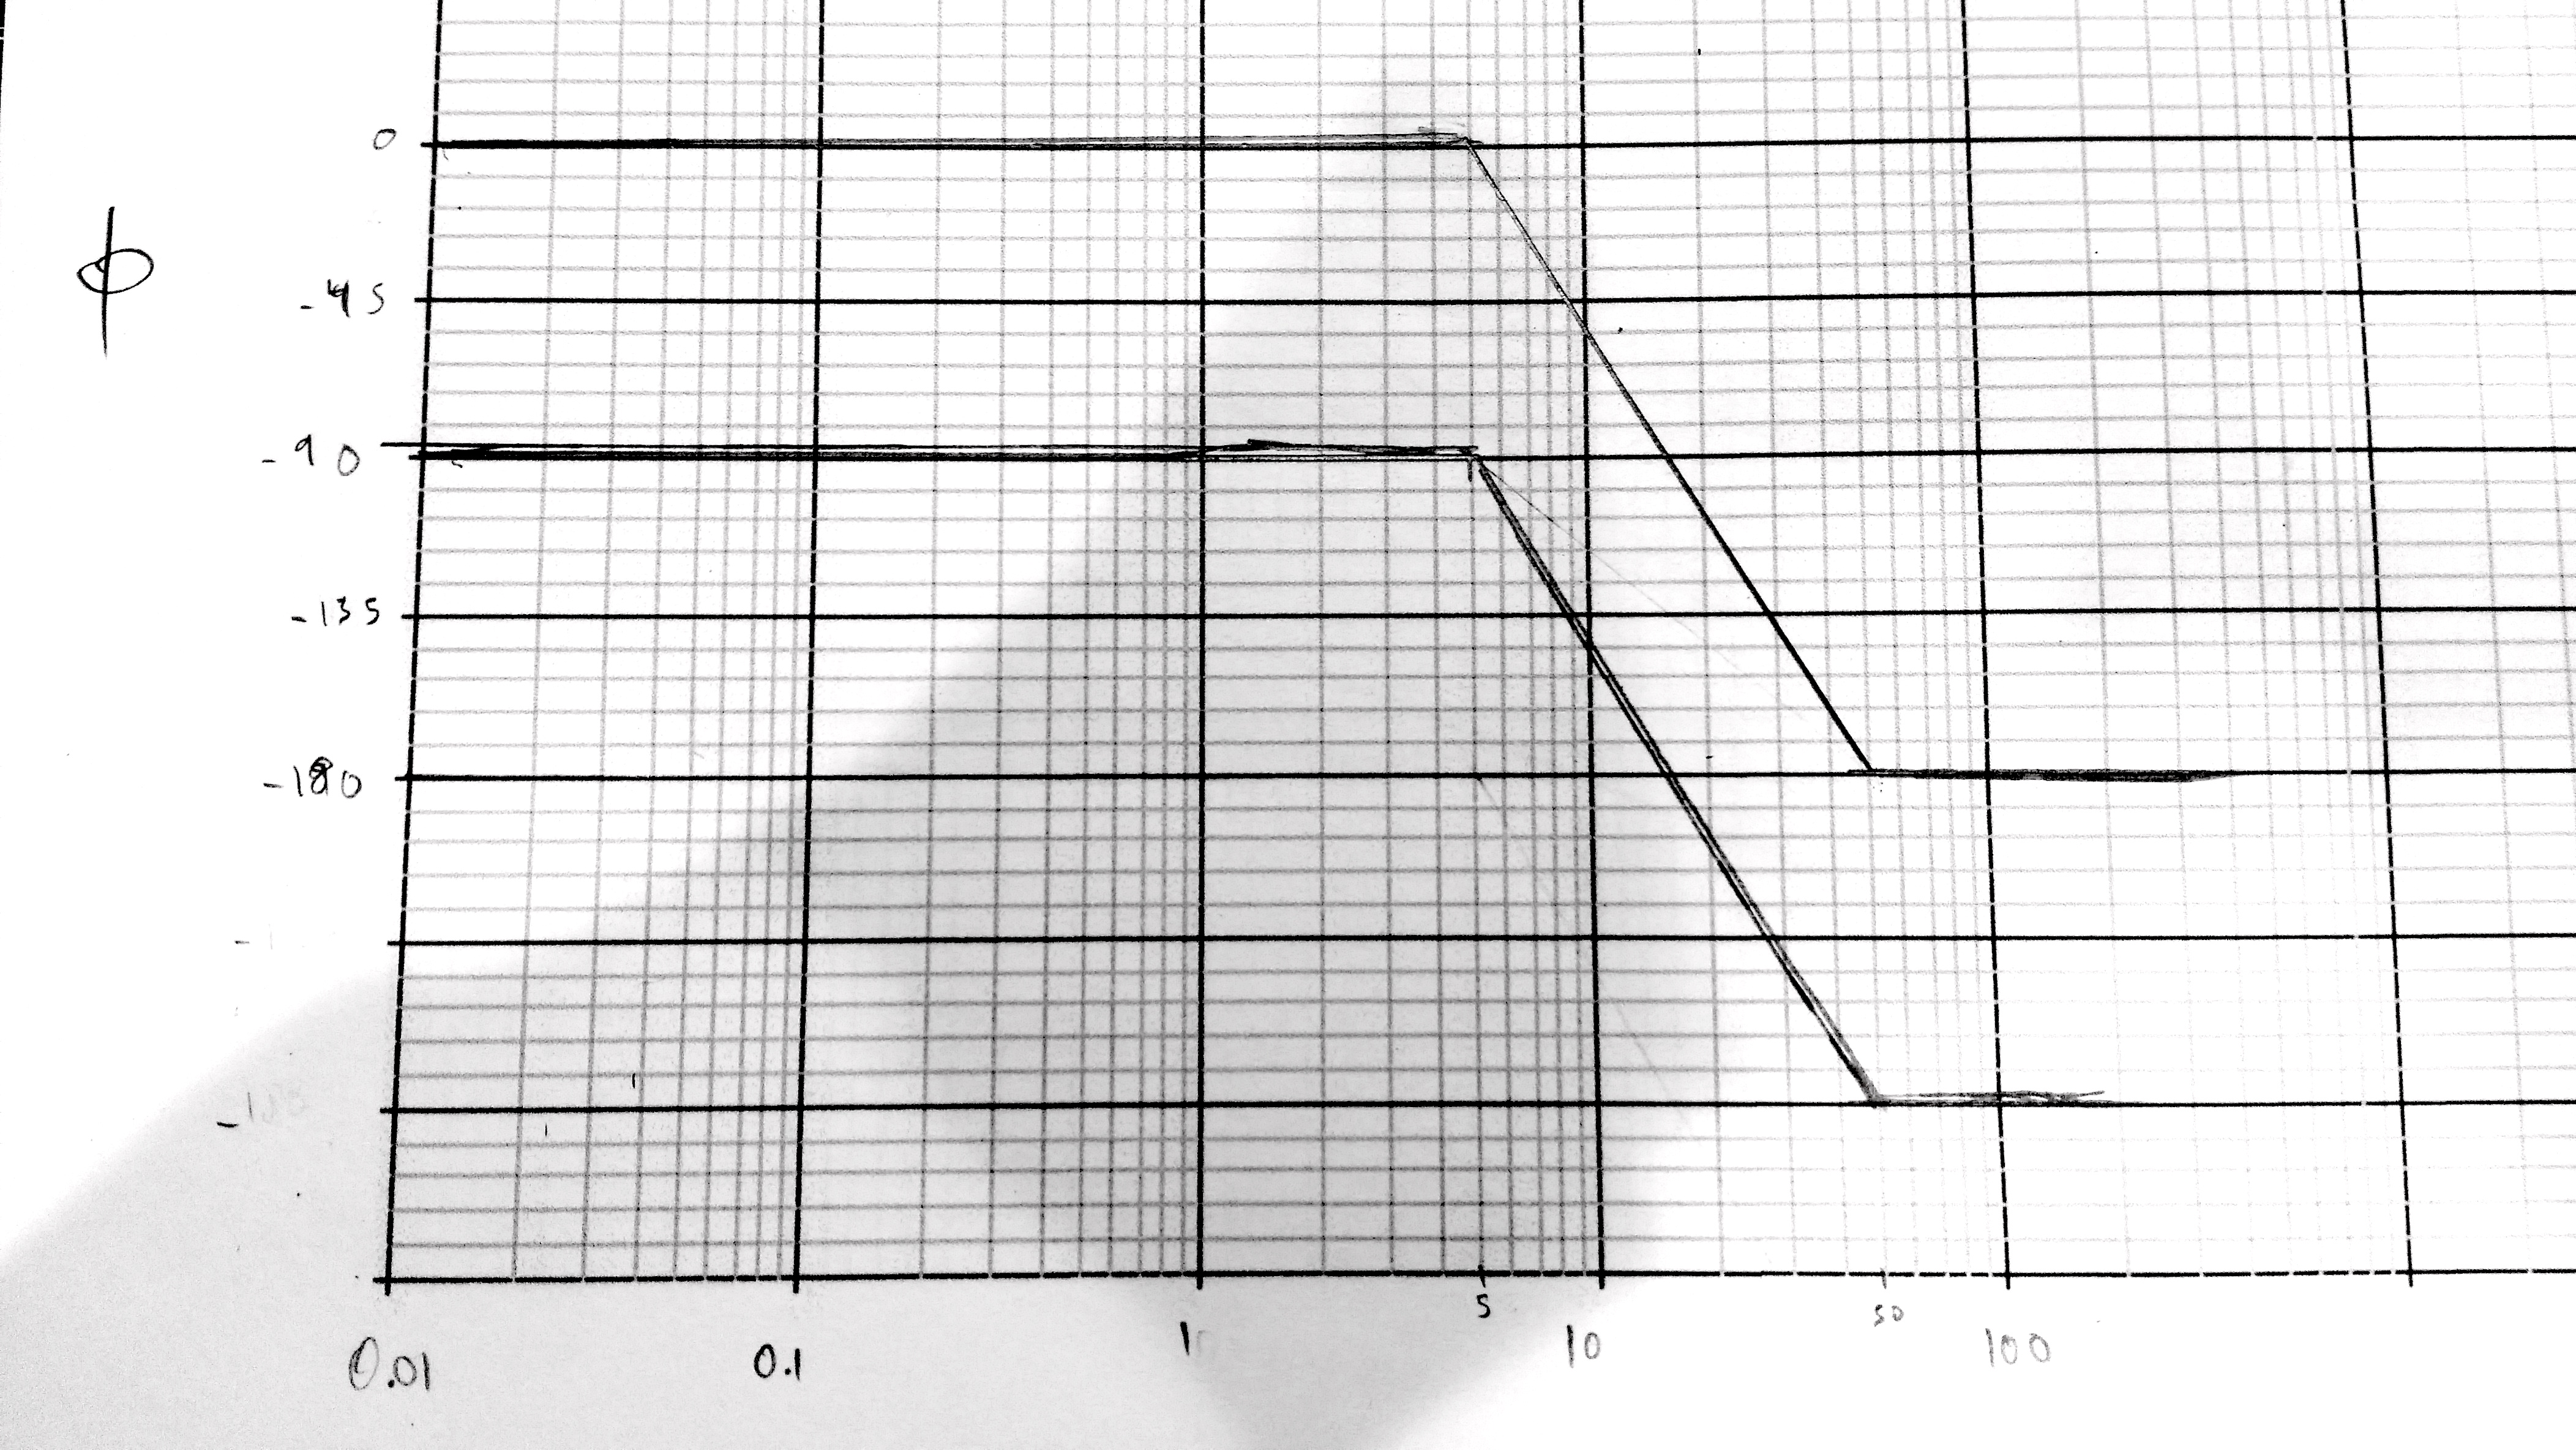
\includegraphics[width=6in]{hand_drawn_bode_plot_phase.jpg} 
   \caption{Hand Performed Bode Plot Phase}
   \label{fig:example}
\end{figure}

\bigskip

The root-locus was then plotted using MATLAB, shown in Figure 4. Note that the hand-drawn plot closely matches the computer generated plot. The Bode plots were also done in MATLAB and are shown in Figure 5. The phase margin and gain margin were found to be 89.725 and 75.0, respectively, which agrees with the values calculated by hand using the RH criterion. 
\bigskip
 
The system was then subjected to a design criteria at which the gain $K = 0.5K_{cr} = 32.5$ and the system's transfer function was determined, as shown in Equation 5. The system's step response at this $K$ was also plotted and the performance criteria calculated, as shown in Figure 6 and Figure 7. It can be seen that the system is stable, however if the gain $K=K_{cr}=75$ then the system is marginally stable for a step response. Any gain $K > 75$ results in the system being unstable.
\bigskip 

\begin{equation}
T = \frac{32.5}{s^3 + 3s^2 + 25s + 32.5}
\end{equation}

 \newpage
 
\begin{figure}[h!] %  figure placement: here, top, bottom, or page
   \centering
   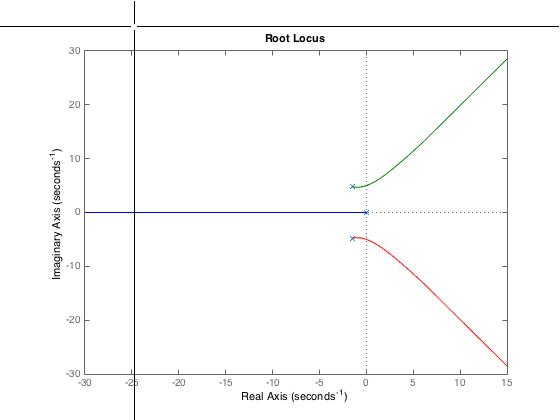
\includegraphics[width=5in]{system_root_locus.jpg} 
   \caption{System Root Locus}
   \label{fig:example}
\end{figure}

\begin{figure}[h!] %  figure placement: here, top, bottom, or page
   \centering
   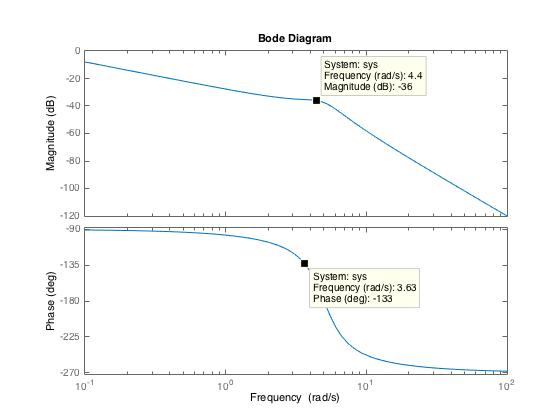
\includegraphics[width=5in]{system_bode_plots.jpg} 
   \caption{System Bode Plots}
   \label{fig:example}
\end{figure}

\newpage

\begin{figure}[h!] %  figure placement: here, top, bottom, or page
   \centering
   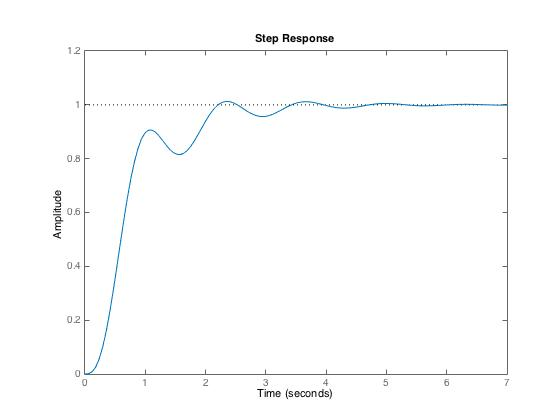
\includegraphics[width=5in]{system_step_resp_half_critical_k.jpg} 
   \caption{Step Response ($K=0.5K_{cr})$}
   \label{fig:example}
\end{figure}

\begin{figure}[h!] %  figure placement: here, top, bottom, or page
   \centering
   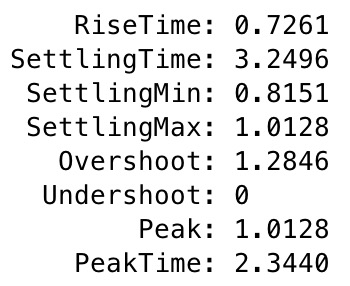
\includegraphics[width=2in]{system_step_info_half_critical_k.jpg} 
   \caption{Step Response Information ($K=0.5K_{cr})$}
   \label{fig:example}
\end{figure}


\section*{\fontsize{12}{12}\selectfont \large Conclusion}
\addcontentsline{toc}{section}{Conclusion} % Add for each section
The exercises conducted in this lab reinforce the theory learned in the classroom. It is shown that the root-locus plot of a system can show much information about the system. It is also shown that the Bode plots for a system can provide information as to how the system responds at different frequencies, for amplitude and phase. With the information obtained from the root-locus and the Bode plots, a system's response behavior can be estimated quite well.




%\section*{\fontsize{12}{12}\selectfont \large References}

\begin{thebibliography}{2}

% Example
%\bibitem{Wagner}
%Ng, K., Wagner, S.W., Camelio, J., Emblom, W.J. (2010). ?Experimental Analysis of Micro Tube
%Hydroforming Process.? Transactions of NAMRC of SME, 38, 577-584.

\end{thebibliography}



%\section*{\fontsize{12}{12}\selectfont APPENDIX}

%\begin{table}[h!]
%  \caption{}
%  \includegraphics[width=\linewidth]{table1.png}
%\end{table}




\end{document}







----------------------------Templates-------------------------------

-------------------------Figure-----------------------

\begin{figure}[h!]  
  \centering
    \includegraphics[width=\linewidth]{**file**}
    \caption{Docking Station}
\end{figure}

---------------------------Table-----------------------
\begin{table}[ht]
\caption{Nonlinear Model Results} % title of Table
\centering % used for centering table
\begin{tabular}{c c c c} % centered columns (4 columns)
\hline\hline %inserts double horizontal lines
Case & Method\#1 & Method\#2 & Method\#3 \\ [0.5ex] % inserts table
%heading
\hline % inserts single horizontal line
1 & 50 & 837 & 970 \\ % inserting body of the table
2 & 47 & 877 & 230 \\
3 & 31 & 25 & 415 \\
4 & 35 & 144 & 2356 \\
5 & 45 & 300 & 556 \\ [1ex] % [1ex] adds vertical space
\hline %inserts single line
\end{tabular}
\label{table:nonlin} % is used to refer this table in the text
\end{table}



probably best to insert as an image from excel

\bigskip\\
\begin{table}[h!]
  \caption{}
  \includegraphics[width=\linewidth]{**file**}
\end{table}
\bigskip\\





-----------------------------Equations------------------------
-----------------------------Regular
\begin{equation}
a = b + c
\end{equation}

--------------------------------- Multiline
\begin{multline}
a = b + c + d + e + f
+ g + h + i + j \\
+ k + l + m + n + o
\end{multline}

-------------------------------Citations-------------------------
\bibitem{Author last name}
  Last, First., year of publication,
  article name, book(etc) name, from \\
  link goes here

----------------------------------other-----------------------------

equations:
http://moser-isi.ethz.ch/docs/typeset_equations.pdf

citations:
http://library.missouri.edu/engineering/about/guides/asme
https://www.asme.org/shop/proceedings/conference-publications/references